\documentclass[12pt]{article}

\usepackage{amsmath, amsthm, amssymb, amsfonts}
\usepackage{derivative, cancel, hyperref, bookmark}
\usepackage[english]{babel}
\usepackage[Rejne]{fncychap}
\usepackage[utf8]{inputenc}
\usepackage[T1]{fontenc}
\usepackage{mathpazo}
\usepackage{caption, subcaption}
\usepackage[dvipsnames]{xcolor}
\usepackage{tcolorbox, color, soul}
\usepackage[a4paper, portrait, margin=1.5cm]{geometry}
\tcbuselibrary{theorems, skins, breakable}
\hypersetup{colorlinks=true, linkcolor=blue, filecolor=magenta, urlcolor=cyan}

\begin{document}

\begin{titlepage}
	\newcommand{\HRule}{\rule{\linewidth}{0.5mm}}
	\center
	
	% Headings
	\textsc{\Huge Systems and Control Engineering}\\[1.5cm]	
	\textsc{\LARGE\bfseries SC649: Embedded Controls and Robotics}\\[1cm] % Major heading
	
	% Title
	\HRule\\[0.4cm]	
	{\huge\bfseries Assignment 1}\\[0.2cm] % Title of your document
	\HRule\\[1.5cm]
	
	% Author(s)
	\begin{minipage}{0.4\textwidth}
		\begin{flushleft}
			\large
			\textit{Team}\\
			\textsc{Pranav Gupta} (\texttt{22B2179})\\
			\textsc{Rohan Mekala} (\texttt{22B2106})\\
			\textsc{Sahil Sudhakar} (\texttt{210010055})\\
		\end{flushleft}
	\end{minipage}
	~
	\begin{minipage}{0.4\textwidth}
		\begin{flushright}
			\large
			\textit{Instructor}\\
			\textsc{Prof. Leena Vachhani}\\
            \href{mailto:leena.vachhani@iitb.ac.in}{leena.vachhani@iitb.ac.in}
		\end{flushright}
	\end{minipage}
	
	% Logo
	\vfill\vfill\vfill
	\includegraphics[width=0.4\textwidth]{/home/pranav/Documents/LaTeX/SysCon/logo.png}\\[1cm]
	
	% Date
	\vfill\vfill
	{\LARGE \today}
	\vfill
	
\end{titlepage}

\pagebreak
\tableofcontents
\pagebreak

\section{Setup}
\begin{enumerate}
    \item We have used \texttt{IN3} and \texttt{IN4} pins of the \textbf{\textbf{L298N}} motor driver to provide differential inputs to the Arduino to rotate the motor in clockwise/anticlockwise direction.
    \item Since we have used \texttt{IN3} and \texttt{IN4}, we have used the \texttt{\texttt{ENB}} pin of the motor driver to provide power to the motor via the Arduino.
    \item \texttt{\texttt{C1}} and \texttt{\texttt{C2}} are the inputs that we receive from the encoder based on the direction of the motor(encoder) rotation.
\end{enumerate}

\begin{figure}[ht!]
    \centering
    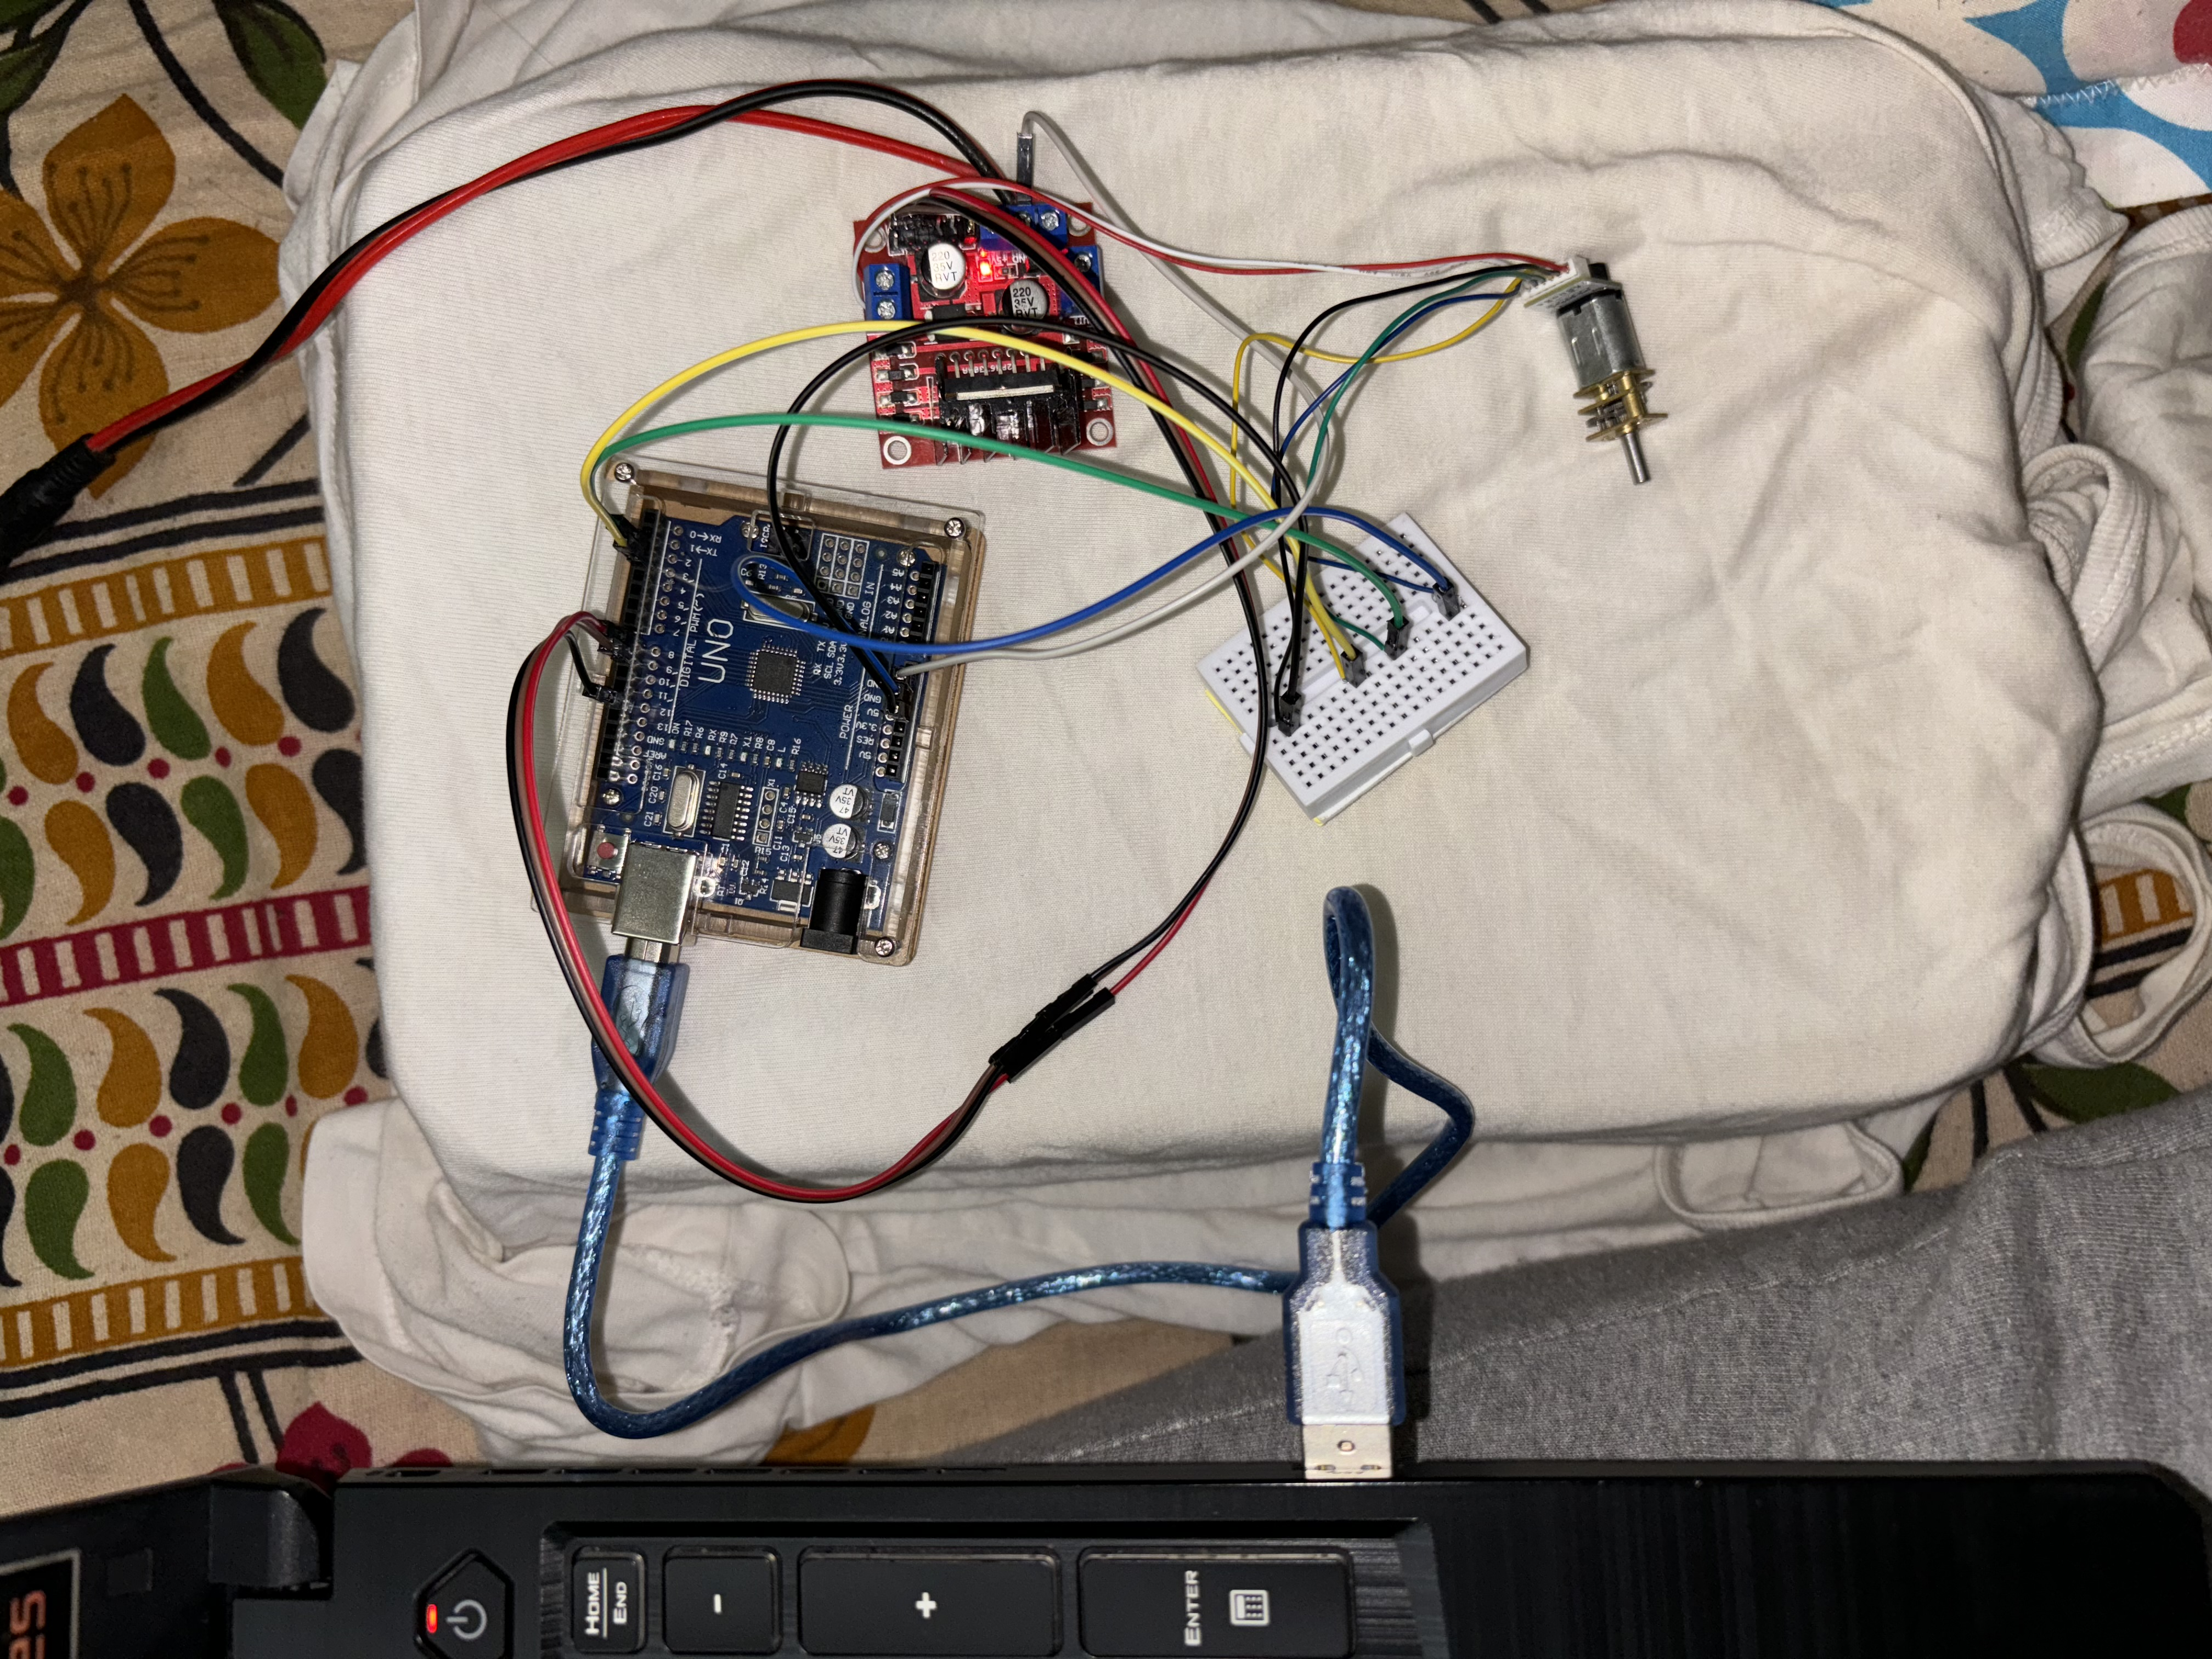
\includegraphics[width=\textwidth]{images/setup.jpeg}
    \caption{photograph of setup}
\end{figure}

\pagebreak
\section{Problem Statement 1}

\subsection{Aim}

Implement an open-loop controller, as shown in Figure 1 to control the speed and direction of the motor.
\begin{enumerate}
    \item Take user input from the serial monitor to determine the direction of motor rotation. You can take input as 1,-1, and 0 for clockwise, anticlockwise rotation, and stopping the motor, respectively.
    \item Take user input from the serial monitor for the required Duty Cycle.
    \item Generate PWM signals based on user input and control the speed and direction of the motor.
    \item Try generating PWM signals at different frequencies and observe the effects on motor behavior. Share your results in detail and your conclusions from it
\end{enumerate}

\subsection{Methodology}
\begin{enumerate}
    \item To take user input from the serial monitor, we used the \texttt{Serial.available()} function to take the user's duty cycle and motor direction inputs.
    \item We have set up a switch case block to allow the user the choice of clockwise rotation, anticlockwise rotation or stopping the motor by inputting 1, -1 and 0 respectively.
    \item For clockwise rotation, “HIGH LOW” input via \texttt{IN3} and \texttt{IN4} is required whereas for anticlockwise rotation, “LOW HIGH” input is required. For stopping the motor, either “LOW LOW” should suffice since the encoder works on a differential input model to decide the direction of rotation.
    \item Along with that, we have also asked the user to input the duty cycle. The assumption we have made here is that the input would be up to 2 decimal places (for eg: 0.25 duty cycle).
    \item To generate PWM signals at different frequencies, we established a logic using the duty cycle. As the duty cycle is \(\frac{T_{on}}{T_{on}+T_{off}}\) and frequency is simply \(\frac{1}{T_{on}+T_{off}}\), we defined a constant \texttt{N} at the start of the code which sets the period of the PWM signal in milliseconds, so that the PWM frequency came out to be \(1000/N\) Hz. We used a for loop that goes from i=1 to i=50/N and in each iteration, we first gave HIGH input through \texttt{\texttt{ENB}}, then placed a delay of \(N*\text{dutycycle}\), which would correspond to \(T_{on}\), then gave Low input through \texttt{\texttt{ENB}} and placed a delay of \(N*(1-\text{dutycycle})\), which would correspond to \(T_{off}\).
\end{enumerate}

\pagebreak
\subsection{Observations}

\begin{figure}[h]
    \centering
    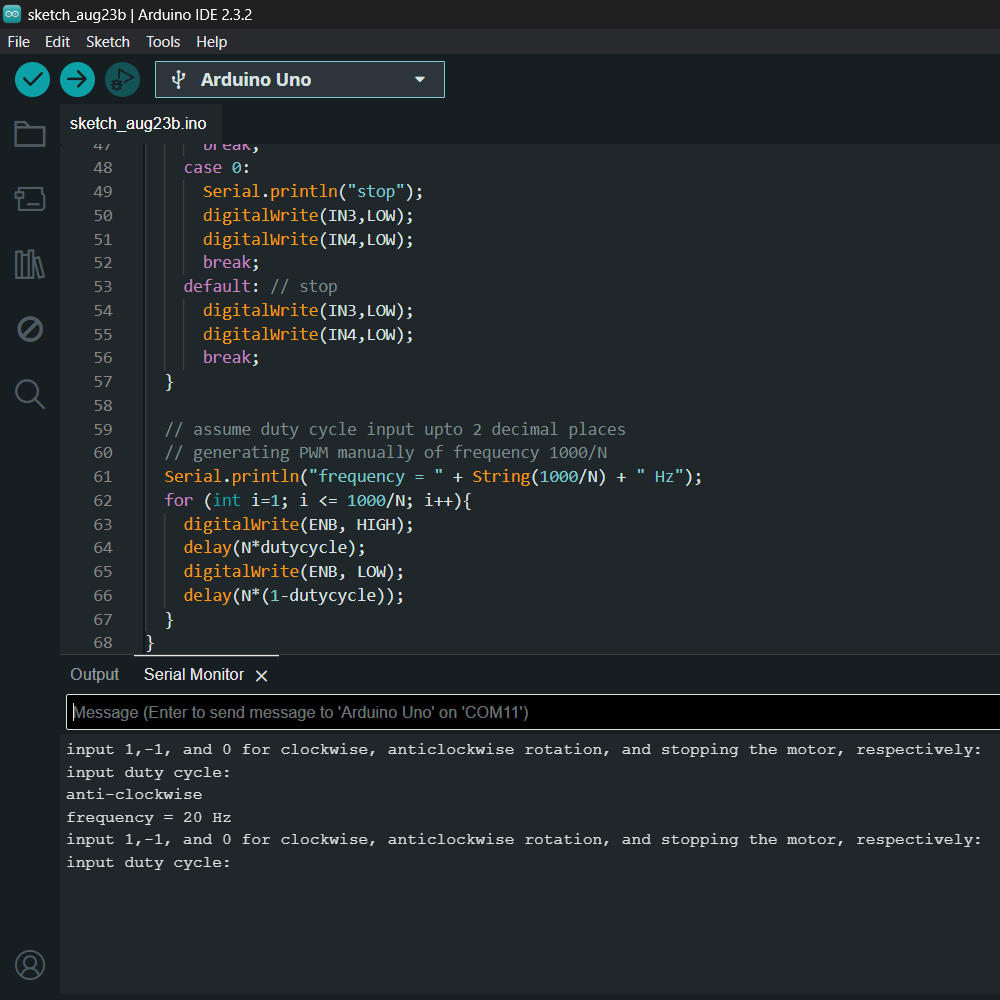
\includegraphics[width=0.8\textwidth]{images/manualpwm.png}
    \caption{Serial Monitor output for taking direction and duty cycle from user and generating PWM signal for motor open loop control manually}
\end{figure}

\subsection{Results \& Conclusions}

By taking user input via the \texttt{Serial.available()} function, we were able to successfully control the direction of the motor by varying the differential inputs via \texttt{IN3} and \texttt{IN4} from “HIGH LOW” to “LOW HIGH” and vice versa and also control the speed of the motor using the duty cycle input by the user. We were able to use the relation between frequency and duty cycle and place appropriate delays between the HIGH and LOW inputs through \texttt{ENB} to vary the PWM frequency.


\pagebreak
\section{Problem Statement 2}

\subsection{Aim}

Interface the encoder with the motor, as shown in Figure 1, and read the data from it
\begin{enumerate}
    \item Do the necessary calculations and calibrations and based on that, calculate the motor RPM and make a map of duty-cycle to encoder count to motor speed(RPM).
    \item Use the encoder data to determine if the motor is rotating clockwise or anticlockwise.
    \item Display the necessary information on the serial monitor
\end{enumerate}

\subsection{Methodology}

\begin{enumerate}
    \item The state of the encoder is the input we get from \texttt{\texttt{C1}} and \texttt{\texttt{C2}}. We have declared variables \texttt{acurr} and \texttt{bcurr} which are the current state of the encoder as they read the input from \texttt{\texttt{C1}} and \texttt{C2} respectively, and \texttt{aprev} and \texttt{bprev} which are the previous state of the encoder. These 4 variables have been initially defined as 0. We have also initialized a variable \texttt{tickCounter} to 0 which will act as our tick counter.
    \item We observed that the \texttt{C1} and \texttt{C2} directional inputs (states) follow a certain pattern
    \begin{itemize}
        \item Clockwise: 00 10 11 01 00
        \item Anticlockwise: 00 01 11 10 00
    \end{itemize}
    \item We have created a nested if structure. The outer if checks whether \texttt{acurr} is different from \texttt{aprev} or \texttt{bcurr} is different from \texttt{bprev}. If either is different, that means the encoder (motor) is rotating, otherwise the \texttt{C1} and \texttt{C2} inputs would simply be 00 00 and so on.
    \item According to our convention, clockwise rotation is negative and anticlockwise rotation is positive.
    \item We have identified that the state pattern for clockwise rotation follows a pattern such that \texttt{acurr} = 1-\texttt{bprev} and \texttt{bcurr} = \texttt{aprev}.
    \item The inner loop checks if this condition is satisfied. If it does, then it is classified as a clockwise rotation and the tick counter is reduced by 1 (since clockwise rotation is negative according to our configuration). If the condition is not satisfied, then it is classified as an anticlockwise rotation and the tick counter is incremented by 1 (since anticlockwise rotation is positive according to our configuration).
    \item At the end of each \texttt{void loop()} iteration, \texttt{aprev} and \texttt{bprev} are given the values of \texttt{acurr} and \texttt{bcurr}.
    \item We marked a line on the encoder and rotated it 50 times and then divided the number of ticks by 50 to get an average estimate of the ticks per encoder rotation which we found to be 25. We defined a variable ticksPerEncoderRotation to store this value.   
    \item To get the ticks per motor rotation, we multiplied the ticks per encoder rotation with the motor shaft gearbox ratio and stored this value in the variable \texttt{ticksPerMotorRotation}.
    \item We have implemented a logic which provides the motor RPM at intervals of 1 second.
    \item We have defined a for loop which has the PWM value as the loop variable which goes from 0 to 255 in steps of 5. We provide this PWM value to the motor via the \texttt{ENB} pin of the \textbf{L298N} motor driver.
    \item For each iteration of this for loop, we have defined a nested for loop which runs 10 times.
    \item In the inner for loop, we have placed a while loop which will execute when \texttt{updateRPM()} returns false. The \texttt{updateRPM()} function uses two variables, currentTime and \texttt{lastUpdateTime}, which we have initially initialised to 0, to keep track of intervals of 1 second. The \texttt{updateRPM()} function does this in the following manner: In void setup(), we have initialised \texttt{lastUpdateTime} to \texttt{millis()}, which is a function which gives us the current system time in milliseconds. In each iteration of the while loop, when \texttt{updateRPM()} function is called at the start of the iteration to check the loop condition, it will return false till the difference between currentTime and \texttt{lastUpdateTime} is lesser than 1 second and in each while iteration, the currentTime variable will be updated using the \texttt{millis()} function and we will also update the number of encoder ticks using the \texttt{updateEncoderTicks()} function which has the same \texttt{tickCounter} logic that we had used in the previous problem statement.
    \item As soon as the difference between currentTime and \texttt{lastUpdateTime} is equal to 1 second, we exit the while loop and we store the value of RPM for that 1 second interval in the \texttt{avgRPM} variable while also dividing by N as we are calculating average RPM.
    \item Here, N is basically the number of 1 second intervals for which we are calculating RPM, adding those values and dividing by N to report the average RPM for N seconds. In our code, we have arbitrarily chosen N to be 10.
    \item So essentially we are incrementing the PWM input from 0 to 255 in steps of 5, and in each iteration, we are calculating 10 RPM values for 10 “1 second intervals” which we are averaging to report the average RPM for that 10 second duration.
    \item In the \texttt{updateRPM()} function, the logic for calculating the RPM for that 1 second interval is as follows: Once a 1 second interval has passed, we will have the updated value of \texttt{tickCounter} variable (with the help of \texttt{updateEncoderTick()} function) which is essentially the \texttt{ticksPerSecond} as our time interval is of 1 second. We then reset the \texttt{tickCounter} value to 0 for the next 1 second interval. We then reset the \texttt{tickCounter} and the \texttt{avgRPM} variable to 0 for the next 1 second interval. We simply multiply the \texttt{ticksPerSecond} with [360/\texttt{ticksPerMotorRotation}] (which is basically the degree of rotation for each tick)  and divide by 60. The \texttt{lastUpdateTime} variable is then given the value of the currentTime variable for the next 1 second interval.
\end{enumerate}

\pagebreak
\subsection{Observations}

\begin{figure}[h]
    \centering
    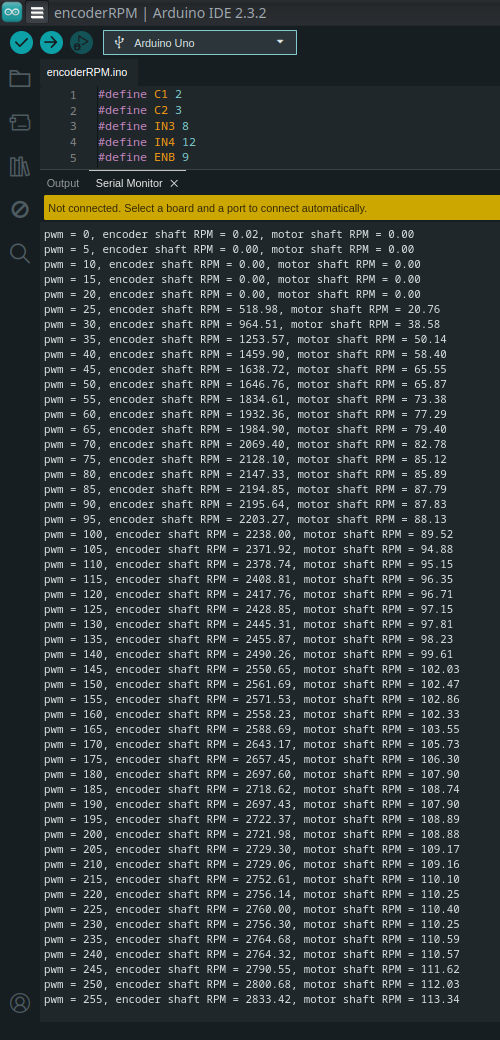
\includegraphics[width=0.5\textwidth]{images/serial-pwm-rpm.png}
    \caption{Serial Monitor output for \texttt{pwm}-\texttt{encoderRPM}-\texttt{motorRPM} mapping}
\end{figure}

\begin{figure}[h]
    \centering
    \begin{subfigure}{.45\textwidth}
        \centering
        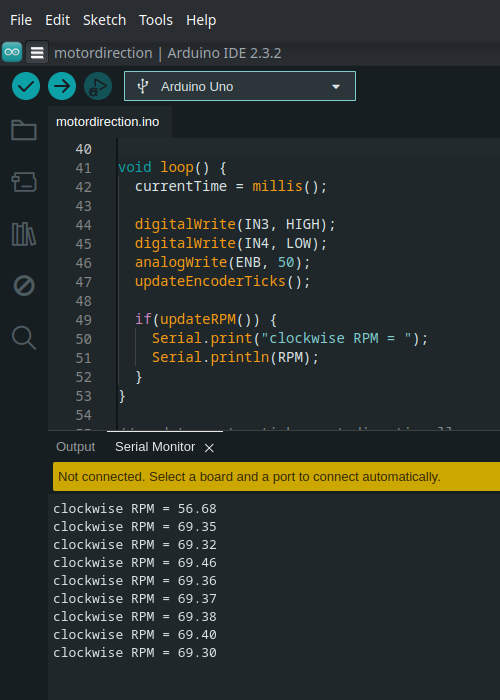
\includegraphics[width=0.75\linewidth]{images/clock.png}
        \caption{clockwise rotation}
    \end{subfigure}
    \begin{subfigure}{.45\textwidth}
        \centering
        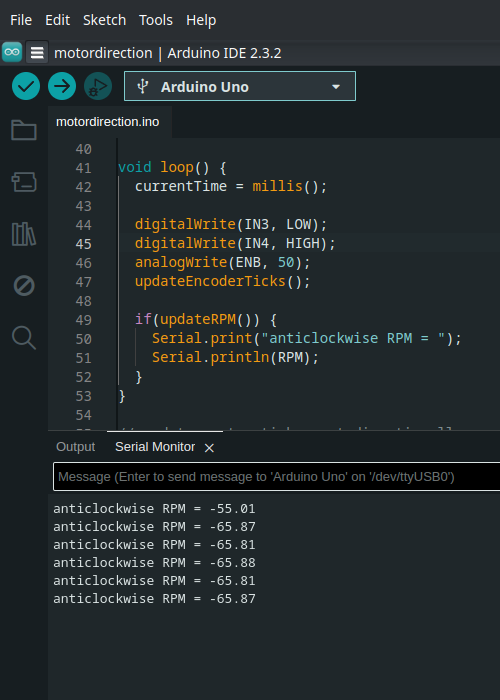
\includegraphics[width=0.75\linewidth]{images/aclock.png}
        \caption{anticlockwise rotation}
    \end{subfigure}
    \caption{Serial Monitor output for detecting motor rotation direction using encoder readings}
\end{figure}

\pagebreak
\subsection{Results}

\begin{figure}[ht!]
    \centering
    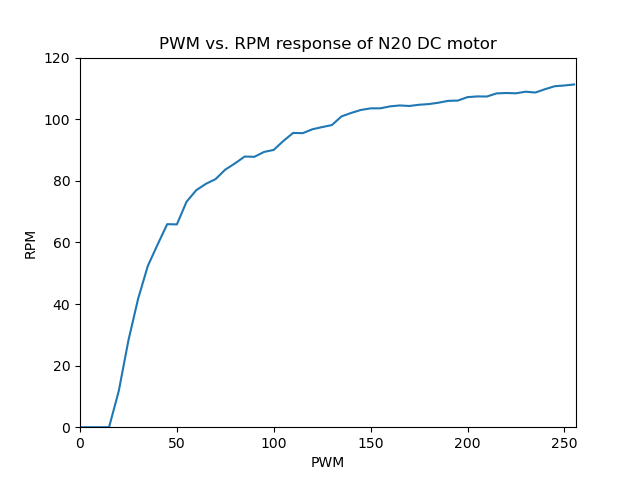
\includegraphics[width=0.6\textwidth]{images/n20.png}
    \caption{plot of duty-cycle to motor shaft RPM response measurements}
\end{figure}

\subsection{Conclusions}

We were able to successfully calculate the RPM of the motor using the 1 second interval logic that we developed. We were able to do so while mapping the duty cycle to the RPM by varying the PWM value from 0 to 255 in steps of 5. In our code, we have calculated the average RPM for 10 “1 second intervals” for each PWM iteration (the outer for loop). We have also successfully used the encoder data to determine if the motor is rotating clockwise or anticlockwise using the encoder state pattern logic (\texttt{acurr}, \texttt{aprev}, \texttt{bcurr} and \texttt{bprev}). We have also been able to map the encoder count to the motor speed(RPM) using the \texttt{updateEncoderTicks()} logic.


\end{document}